Conditional Random Fields are best known for their ability to predict optimal configurations of multiple interdependent variables, which in case of semantic image segmentation are pixels or superpixels. The importance of relations between adjacent superpixels was already presented in the previous chapter, though only in terms of the pairwise potential. In this chapter the usage of contextual data also in the local potential will be described as the goal of this part of the system is to differentiate objects by their shape. In the dataset for the experiments of this part of the system an object looking like a letter H was introduced. This object is always in the shades of red and is surrounded by greenish superpixels. In order to prove that indeed the shape of the object is recognised, also squares and circles were involved in the dataset, which base colour and colours of the surroundings are the same as in case of the letter H. Figure \ref{fig:nonlinear_goal} depicts three sample objects that differ only by their shape together with images representing the results of the segmentation process that are to be obtained. 
\begin{figure}[ht]
    \centering
    \begin{tabular}{ccc}
        \fcolorbox{black}{white}{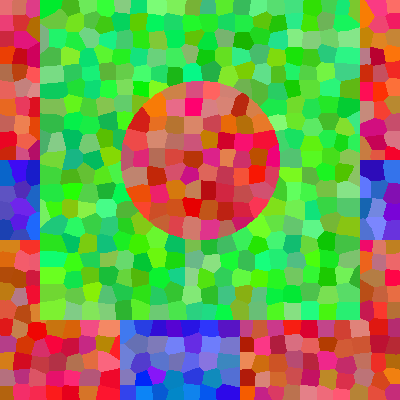
\includegraphics[width = 0.28\textwidth]{nonlinear_intro/circle.png}} &
        \fcolorbox{black}{white}{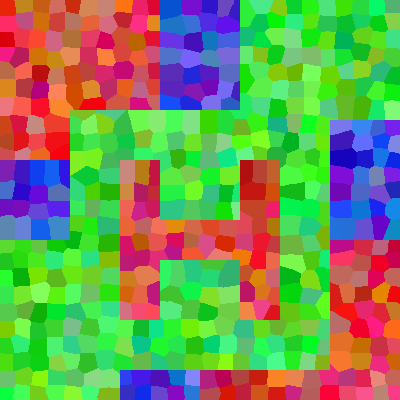
\includegraphics[width = 0.28\textwidth]{nonlinear_intro/letter_h.png}} &
        \fcolorbox{black}{white}{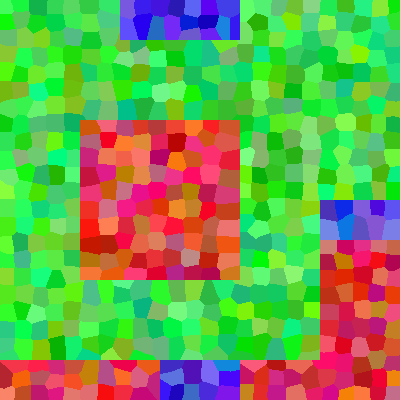
\includegraphics[width = 0.28\textwidth]{nonlinear_intro/square.png}} 
        \\
        \fcolorbox{black}{white}{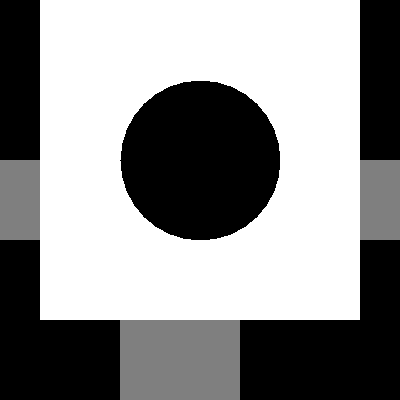
\includegraphics[width = 0.28\textwidth]{nonlinear_intro/circle_N.png}} &
        \fcolorbox{black}{white}{
\includegraphics[width = 0.28\textwidth]{nonlinear_intro/letter_h_N.png}} &
        \fcolorbox{black}{white}{
\includegraphics[width = 0.28\textwidth]{nonlinear_intro/square_N.png}} 
    \end{tabular}
    \caption{Sample images that are to be differentiated basing on their shape and their expected labellings.}
    \label{fig:nonlinear_goal}
\end{figure}
Similarly as before, label 0 is the class for reddish superpixels, label 1 for greenish and label 2 for those in the shades of blue, however, this time another class was introduced, denoted as label 3, which is devoted only to the objects with a shape of letter H.

